\section{Analyse des Fonctionnalités et Résultats de la Page React}

\subsection{Fonctionnalités de la Page React}
La page React développée permet d'analyser les résultats des parties de Tron jouées par les algorithmes. Elle repose sur le chargement d'un fichier JSON généré après chaque partie, et offre plusieurs fonctionnalités pour visualiser et interpréter les performances des IA. \\
\textbf{1. Chargement et Analyse des Données}
\begin{itemize}
    \item La page accepte un fichier JSON contenant les données de la partie.
    \item Elle extrait et affiche les statistiques des joueurs sous forme de graphiques et de timeline.
\end{itemize}

\begin{figure}[h]
	\centering
	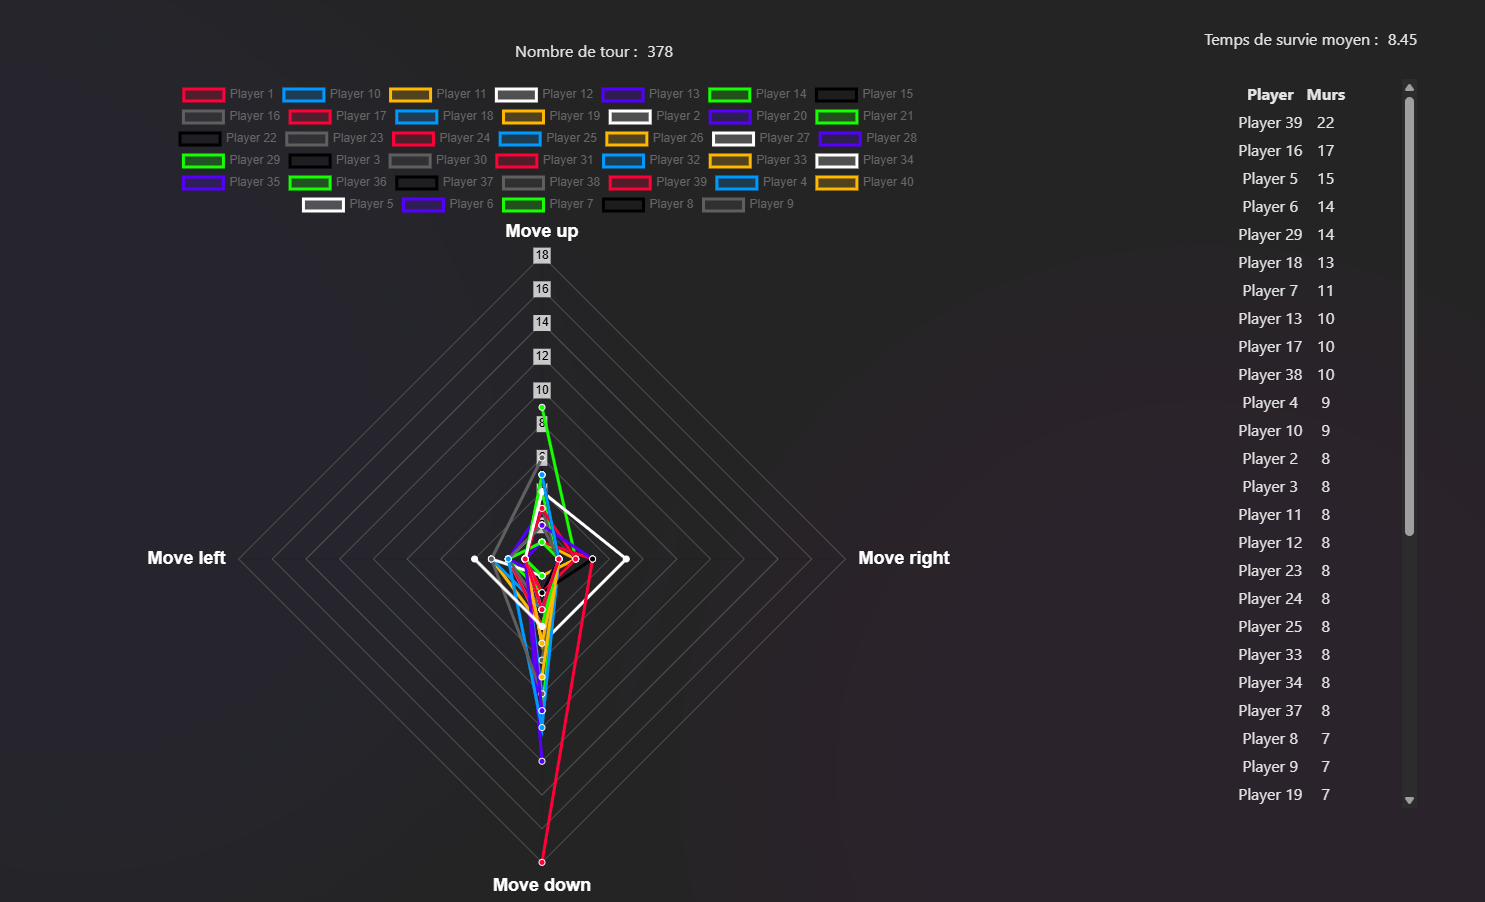
\includegraphics[width=0.8\textwidth]{images/TendanceDeplacement.png}
	\caption{Visualisation des Tendances de Déplacement}
	\label{TendanceDeplacement}
\end{figure}
\textbf{2. Visualisation des Tendances de Déplacement}
\begin{itemize}
    \item Un graphique radar montre les moyennes des mouvements effectués par chaque joueur.
    \item Les tendances de déplacement sont représentées pour comparer le comportement des IA.
    \item Il est possible d'afficher ou masquer les statistiques d'un joueur en activant/désactivant son affichage.
\end{itemize}

\newpage

\begin{figure}[h]
	\centering
	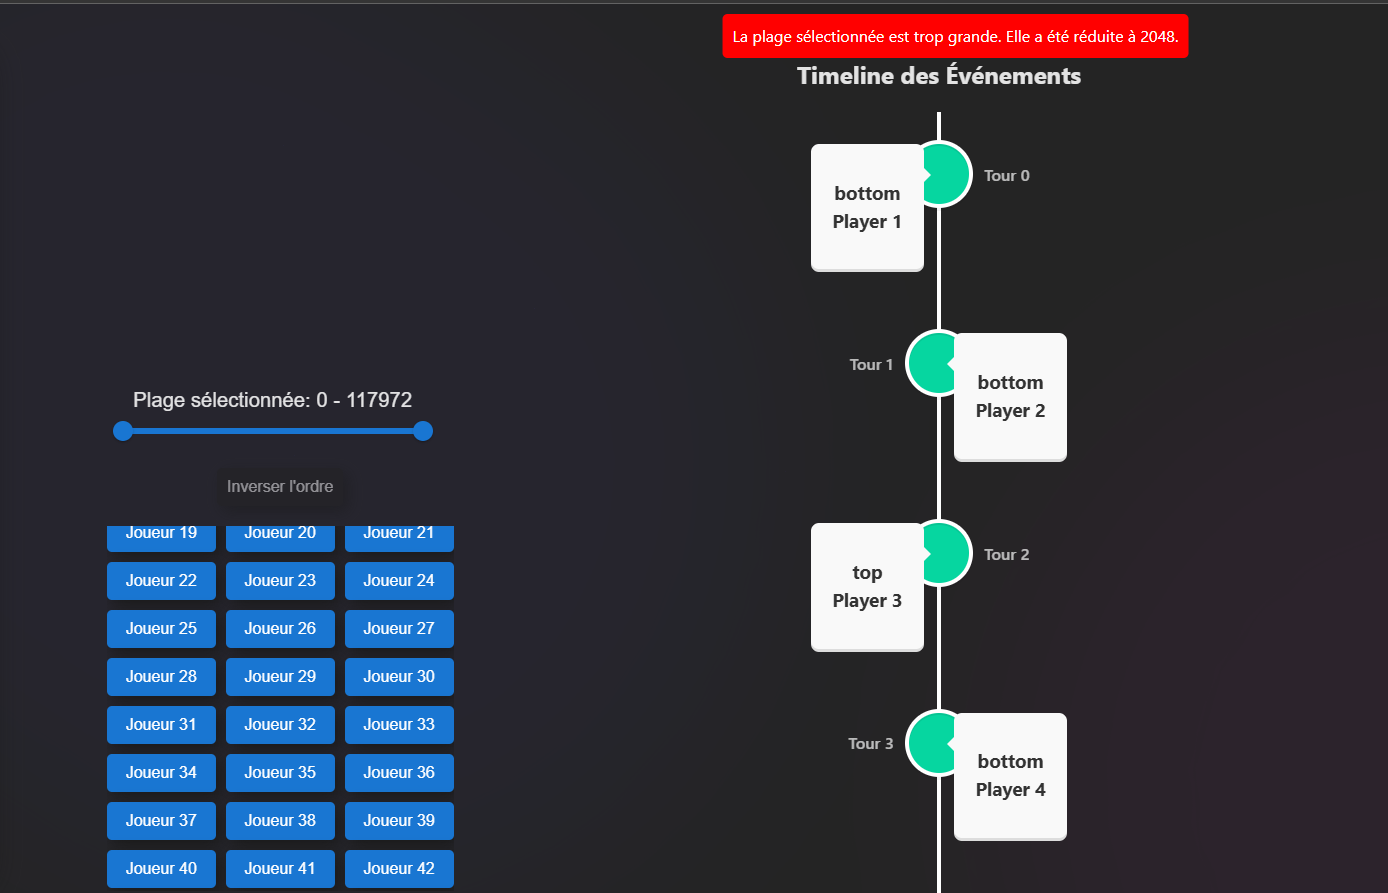
\includegraphics[width=0.7\textwidth]{images/TimelineActions.png}
	\caption{Timeline des Actions}
	\label{TimelineActions}
\end{figure}
\textbf{3. Timeline des Actions}
\begin{itemize}
    \item Une seconde page permet de voir les actions des joueurs tour par tour.
    \item Un curseur permet de sélectionner une plage de tours à afficher.
    \item Les actions peuvent être filtrées par les joueurs.
\end{itemize}

\begin{figure}[h]
	\centering
	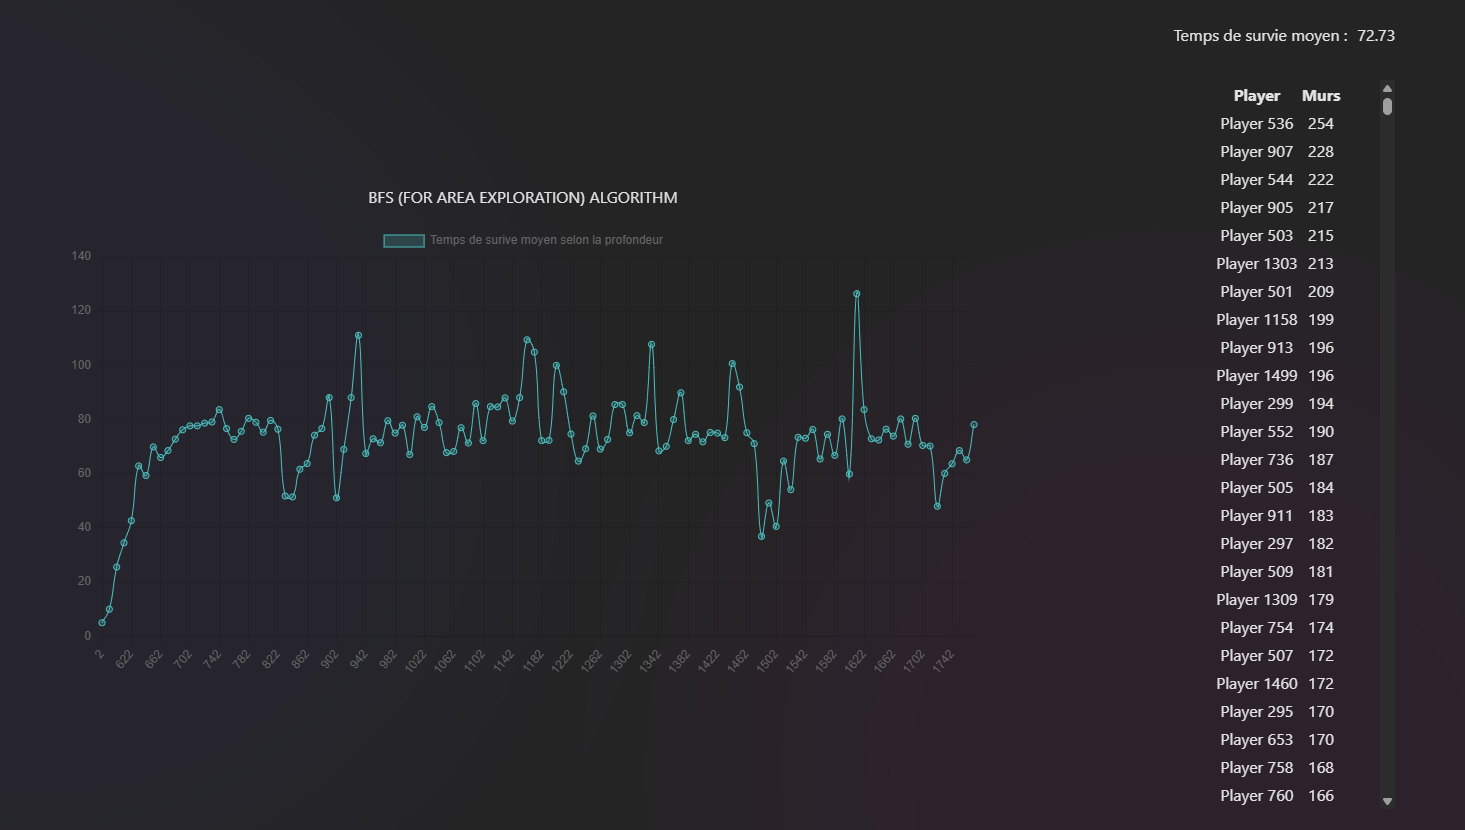
\includegraphics[width=0.7\textwidth]{images/SurvieMoyenProfondeur.png}
	\caption{Temps de Survie Moyen selon la Profondeur de Recherche}
	\label{SurvieMoyenProfondeur}
\end{figure}
\textbf{4. Temps de Survie Moyen selon la Profondeur de Recherche}
\begin{itemize}
    \item Un graphique linéaire affiche l'évolution du temps de survie moyen en fonction de la profondeur de recherche des algorithmes.
    \item Cela permet d'analyser l'impact de la profondeur de recherche sur la performance des joueurs.
\end{itemize}

\subsection{Analyse des Résultats}
L'analyse des parties jouées par les algorithmes met en lumière plusieurs tendances récurrentes dans leur comportement, ainsi que des observations intéressantes sur les performances en fonction de la profondeur de recherche.
\subsubsection{Identification d'un Seuil d'Exploration}
L’un des premiers constats issus de notre analyse est que les algorithmes ont tendance à adopter des schémas de déplacement optimisés pour éviter les conflits entre joueurs. Quel que soit l’algorithme utilisé (MAXN, Paranoid, SOS ou BFS), on observe une forte propension à évoluer en ligne droite, souvent en synchronisation avec les autres joueurs, en alternant des mouvements de gauche à droite ou d’avant en arrière. \\
Ce phénomène s’explique par le fait que ces déplacements permettent aux agents d’exploiter l’espace de manière rationnelle en minimisant les risques de collision et en maximisant le contrôle de leur zone de jeu. Ainsi, même sans coordination explicite entre eux, les joueurs adoptent des comportements qui rappellent des stratégies collaboratives, où chacun cherche à préserver son propre espace sans perturber les trajectoires des autres. \\
Cependant, nous avons remarqué que cette stratégie atteint une limite lorsque les joueurs sont trop nombreux ou que l’espace devient restreint. Une fois ce seuil d’exploration dépassé, les IA doivent adopter des mouvements plus erratiques et commencent à s’éliminer plus rapidement.

\subsubsection{Mesure des Performances en Fonction de la Profondeur}
L’un des éléments clés de notre analyse repose sur l’étude du temps de survie moyen des joueurs en fonction de la profondeur de recherche de l’algorithme. Le graphique généré met en évidence plusieurs tendances :
\begin{itemize}
    \item À faible profondeur, les IA prennent des décisions rapides mais manquent d’anticipation, ce qui conduit souvent à des éliminations précoces.
    \item En augmentant la profondeur de recherche, on observe une nette amélioration du temps de survie moyen, car les joueurs parviennent à mieux anticiper les menaces et à optimiser leurs déplacements.
    \item Toutefois, passé un certain seuil, l’amélioration devient moins significative et peut même se dégrader dans certains cas. 
\end{itemize}
Cette observation suggère qu’il existe un compromis à trouver entre la profondeur d’exploration et la rapidité d’exécution, afin d’optimiser la performance des joueurs sans alourdir inutilement les calculs.

\newpage

\subsubsection{Équilibre entre Coût et Gain Stratégique}
Le principal défi des algorithmes utilisés réside dans l’équilibre entre le coût de calcul et le gain stratégique obtenu. Nos observations montrent que si une recherche trop superficielle entraîne des décisions sous-optimales, une profondeur excessive ne garantit pas forcément un avantage déterminant. \\
Ce constat est particulièrement visible avec les algorithmes comme Paranoid et MAXN, qui nécessitent une grande puissance de calcul pour évaluer plusieurs niveaux de jeu. À l’inverse, BFS, bien qu’explorant un grand nombre de possibilités, peut parfois être pénalisé par sa manière d’étendre l’arbre de décision. \\
En pratique, le choix du paramètre de profondeur doit être ajusté en fonction du contexte de la partie et des ressources disponibles. Une future amélioration pourrait être d’adapter dynamiquement cette profondeur en fonction des situations rencontrées, afin d’optimiser en temps réel l’équilibre entre réactivité et stratégie à long terme.

\subsubsection{Comparaison des Algorithmes}
L’analyse des résultats met en évidence des différences marquées entre les algorithmes étudiés, que ce soit en termes de stratégie adoptée, de performance en fonction de la profondeur ou d’optimisation du temps de calcul.
\paragraph{MAXN}
L’algorithme MAXN, conçu pour les jeux multi-joueurs, cherche à maximiser le score de chaque agent sans nécessairement chercher à bloquer les autres. On observe qu’à profondeur faible, il produit des trajectoires relativement naïves, mais dès qu’on augmente la profondeur, il adopte des déplacements plus optimisés et coordonnés, avec une meilleure gestion de l’espace. Cependant, il devient coûteux en calcul avec une profondeur élevée, ce qui limite son efficacité en temps réel.
\paragraph{Paranoid}
Contrairement à MAXN, l’algorithme Paranoid fonctionne sur un principe plus compétitif en considérant que tous les autres joueurs sont adversaires. Cela le pousse à être plus agressif dans ses décisions, essayant activement d’enfermer ses concurrents ou de bloquer leur progression. Toutefois, cette approche peut parfois être trop risquée, menant à des éliminations rapides si un joueur se retrouve trop tôt dans un espace clos.
\paragraph{SOS}
L’algorithme SOS adopte une approche plus équilibrée, cherchant à maximiser son propre espace disponible tout en minimisant celui des autres. Il génère ainsi des comportements qui semblent plus "prudents" que ceux de Paranoid, mais moins optimisés que MAXN sur le long terme. Il est intéressant de noter que SOS est particulièrement efficace lorsque la grille est encore ouverte, mais devient moins performant en fin de partie où une adaptation plus fine est nécessaire.
\newpage
\paragraph{BFS}
BFS, utilisé ici pour l’exploration du terrain, offre une approche plus déterministe, cherchant avant tout à couvrir un maximum d’espace sans forcément anticiper les actions des autres joueurs. Il donne des résultats cohérents mais peut être pénalisé par un manque de prise en compte des adversaires. Son avantage principal est sa rapidité d’exécution et sa robustesse à faible profondeur, mais il peine à rivaliser avec MAXN ou Paranoid lorsqu’on cherche une optimisation stratégique avancée.
\paragraph{Conclusion}
Chaque algorithme présente des forces et des faiblesses selon le contexte de la partie. MAXN offre la meilleure optimisation stratégique mais est gourmand en calcul, Paranoid est agressif mais risqué, SOS est équilibré mais manque d’adaptabilité en fin de partie, et BFS est rapide mais limité en termes de prise de décision stratégique.

Une amélioration future pourrait être d’hybrider ces approches, en utilisant par exemple une stratégie adaptative qui change de méthode en fonction de la situation sur la grille.
